\section{Hypothesised outcome} \label{hypothesis} 

The proposed hypothesis is that the Clean Architecture approach can be applied in
conjunction with the Normalized Systems theorems. The design principles of Clean
Architecture converge with the theorems of Normalized Systems. Consequently, the artifact
that is part of this design research will lead to a highly modular, stable, and evolvable
C\# artifact that does not contradict Normalized Systems theorems.

Both architectural approaches formulate modular structures independent of any programming
technology \parencite{mannaert_normalized_2009,robert_c_martin_clean_2018}. As such, the
C\# artifact produced as part of this research has similar trademarks of modularity,
evolvability, and stability compared to case studies where Java SE has been used.
\parencite{oorts_building_2014, de_bruyn_enabling_2018}. Furthermore, applicability of
Clean Architecture has no additional or negative effect when used in conjunction with the
Normalized Systems Theorems.

\begin{figure}[H]
    \centering
    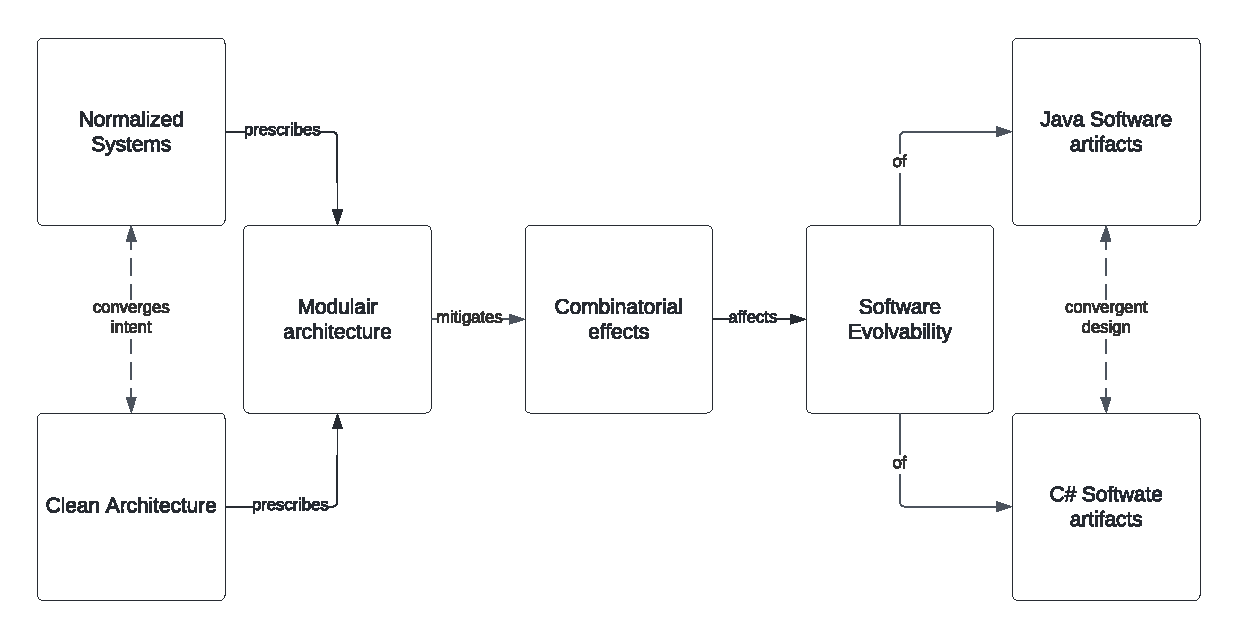
\includegraphics[width=0.8\textwidth]{Figures/hypothesis.pdf}
    \caption[The hypothesis]{The hypothesis}
    \label{fig_hypothesis}
\end{figure}